\documentclass{article}

% Soporte para Unicode.
% En vez de usar pdflatex, usa el comando xelatex.

\usepackage{fontspec}
\setmainfont{Latin Modern Roman}
\setmonofont{JetBrains Mono}

\usepackage[margin=1in]{geometry} % márgenes de la página
\usepackage{enumitem} % para listas personalizadas
\usepackage{fancyhdr} % para encabezados y pies de página
\usepackage[table]{xcolor} % para colores en tablas
\usepackage{xcolor} % para colores personalizados
\usepackage{hyperref} % para enlaces
\usepackage{tikz} % para dibujar diagramas (AFD)
\usepackage{tcolorbox} % para cajas de texto
\usepackage{indentfirst} % para la sangría al iniciar una sección
\usepackage{listings} % para los códigos del anexo

\setlength{\headheight}{13.07225pt}
\addtolength{\topmargin}{-1.07225pt}

\pagestyle{fancy}
\fancyhead[L]{Grupo 7}
\fancyhead[C]{}
\fancyfoot[L]{Práctica 1 - Procesadores de Lenguajes}
\fancyfoot[C]{}
\fancyfoot[R]{\thepage}

\title{\textbf{Práctica 1 - Procesadores de Lenguajes}}
\author{\textbf{Grupo 7}\\Carmen Toribio Pérez, 22M009\\Sergio Gil Atienza, 22M046\\María Moronta Carrión, 22M111}
\date{}

\begin{document}

\maketitle

\section{Introducción}

La primera entrega de esta práctica consiste en la implementación de un Analizador Léxico y una Tabla de Símbolos. Para ello, hemos seguido los siguientes pasos: 
\begin{enumerate}
    \item \textbf{Identificar los Tokens} del lenguaje fuente, teniendo en cuenta las especificaciones de nuestro grupo.
    \item Construir la \textbf{Gramática Regular} que los genera.
    \item Diseñar el \textbf{Autómata Finito Determinista} equivalente a la gramática. Hemos realizado una representación de este a través de un \textbf{diagrama de estados}.
    \item Añadir las \textbf{Acciones Semánticas}, asociadas a cada una de las transiciones del diagrama de estados.
    \item Estudiar los posibles \textbf{casos de error}, para poder manejar correctamente la detección y el reporte de errores léxicos. 
\end{enumerate}

Por otro lado, hemos comenzado con la implementación de la \textbf{Tabla de Símbolos}, concretamente con el diseño de su estructura y su organización.\\

Finalmente, presentamos una serie de casos de prueba que demuestran el correcto funcionamiento del Procesador, así como su capacidad para manejar errores léxicos.\\

Como integrantes del \textbf{grupo 7}, hemos tenido que cumplir con las siguientes especificaciones: 
\begin{itemize}[left=2cm]
    \item Sentencias: Sentencia repetitiva (for)
    \item Operadores especiales: Asignación con suma (+=)
    \item Técnicas de Análisis Sintáctico: Descendente Recursivo
    \item Comentarios: Comentario de bloque (/* */)
    \item Cadenas: Con comillas simples (' ')
\end{itemize}

Hemos decidido usar C++ como lenguaje de programación ya que la mayor parte de la infraestructura de compiladores está escrita en C o en C++, incluyendo MSVC (desarrollado por Microsoft) y el proyecto LLVM (utilizado por Google en Android). También hemos tenido en cuenta su flexibilidad y potencia, junto a la amplia variedad de utilidades que tiene su librería estándar. En comparación con lenguajes como Java o JavaScript, C++ ofrece mayor eficiencia y control sobre los recursos del sistema, a la vez que se mantiene versátil y permite escribir código legible.

\newpage

\section{Tokens}
El primer paso a la hora de construir un Analizador Léxico es la identificación de los tokens. Para hacer la lista nos hemos basado en la actividad práctica de la plataforma Draco. Hemos decidido utilizar el mismo formato en tablas con tal de facilitar su legibilidad.\\
Tokens obligatorios:

\begin{table}[h!]
    \centering
    \begin{tabular}{|l|l|l|}
        \hline
		\rowcolor{gray!20} % color grisaceo en la cabecera de la tabla
        \textbf{Elemento} & \textbf{Código de Token} & \textbf{Atributo} \\ \hline
        boolean & bool & - \\ \hline
        for & for & - \\ \hline
        function & fn & - \\ \hline
        if & if & - \\ \hline
        input & in & - \\ \hline
        int & int & - \\ \hline
        output & out & - \\ \hline
        return & ret & - \\ \hline
        string & str & - \\ \hline
        var & var & - \\ \hline
        void & void & - \\ \hline
        constante entera & cint & Número \\ \hline
        Cadena (') & cstr & Cadena ("c*") \\ \hline
		Identificador & id & Número (posición en la TS) \\ \hline
        += & cumass & - \\ \hline
        = & ass & - \\ \hline
        , & com & - \\ \hline
        ; & scol & - \\ \hline
        ( & po & - \\ \hline
        ) & pc & - \\ \hline
        \{ & cbo & - \\ \hline
        \} & cbc & - \\ \hline
    \end{tabular}
\end{table}

Tokens de operadores aritméticos, lógicos y relcionales:
\begin{table}[h!]
    \centering
    \begin{tabular}{|l|l|l|}
        \hline
		\rowcolor{gray!20} % color grisaceo en la cabecera de la tabla
        \textbf{Grupo de Opciones} & \textbf{Código de Token} & \textbf{Atributo} \\ \hline
        Grupo Operadores Aritméticos: Suma (+) & sum & - \\ \hline
        Grupo Operadores Aritméticos: Resta (-) & sub & - \\ \hline
        Grupo Operadores Lógicos: Y lógico (\&\&) & and & - \\ \hline
        Grupo Operadores Lógicos: O lógico (\texttt{||}) & or & - \\ \hline
        Grupo Operadores Relacionales: Menor (\textless) & ls & - \\ \hline
        Grupo Operadores Relacionales: Mayor (\textgreater) & gr & - \\ \hline
    \end{tabular}
\end{table}

Tokens opcionales:
\begin{table}[h!]
    \centering
    \begin{tabular}{|l|l|l|}
        \hline
		\rowcolor{gray!20} % color grisaceo en la cabecera de la tabla
        \textbf{Grupo de Opciones} & \textbf{Código de Token} & \textbf{Atributo} \\ \hline
        Menos Unario (-) & sub & - \\ \hline
        Más Unario (+) & sum & - \\ \hline
        false & cap & - \\ \hline
        true & nocap & - \\ \hline
        EOF & eof & - \\ \hline
    \end{tabular}
\end{table}

Por tanto, los siguientes tipos de expresiones no serán identificados como tokens: los delimitadores (como los espacios en blanco o las tabulaciones), los comentarios de bloque (/* */) o los saltos de línea (\textbackslash n).

\section{Gramática Regular}

En esta sección, describimos la Gramática Regular (gramática de tipo 3 según la jerarquía de Chomsky) que hemos diseñado para identificar y generar los tokens del lenguaje fuente. 

\begin{center}
    \begin{tcolorbox}[title=Símbolos no terminales, width=0.57\textwidth]
        $d$ := 0...9
        
        $l$ := a..z, A...Z
        
        $c_1$ := espacio o cualquier carácter imprimible menos \textbackslash
        
        $cesc$ := carácter escapable (', 0, n, a, t, v, f, r, \textbackslash )
        
        $c_2$ := cualquier carácter menos * y eof
        
        $c_3$ := cualquier carácter menos *, / y eof
    \end{tcolorbox}
\end{center}

\begin{tcolorbox}[title=Gramática Regular]
    \hspace{0.5cm} S → del S \texttt{|} $l$A \texttt{|} $d$B \texttt{|} 'C \texttt{|} +D\texttt{|} - \texttt{|} = \texttt{|} \(>\) \texttt{|} \(<\) \texttt{|} \&E \texttt{|} \texttt{|}F \texttt{|} /G \texttt{|} \} \texttt{|} \{ \texttt{|} ) \texttt{|} ( \texttt{|} ; \texttt{|} , \texttt{|} eof
    
    \hspace{0.5cm} A → $l$A \texttt{|} $d$A \texttt{|} \_A \texttt{|} \( \lambda \)
    
    \hspace{0.5cm} B → $d$B \texttt{|} \( \lambda \)
    
    \hspace{0.5cm} C → $c_1$C \texttt{|} \textbackslash C' \texttt{|} '
    
    \hspace{0.5cm} C' → $cesc$C
    
    \hspace{0.5cm} D → = \texttt{|} \( \lambda \)
    
    \hspace{0.5cm} E → \&
    
    \hspace{0.5cm} F → \texttt{|}
    
    \hspace{0.5cm} G → *H
    
    \hspace{0.5cm} H → $c_2$H \texttt{|} *I
    
    \hspace{0.5cm} I → /S \texttt{|} $c_3$H \texttt{|} *I
\end{tcolorbox}

\section{Autómata Finito Determinista}
Una vez definida la gramática regular, el siguiente paso es construir el Autómata Finito Determinista (AFD) correspondiente. A continuación, presentamos su diseño, incluyendo las transiciones entre estados.

\begin{center}
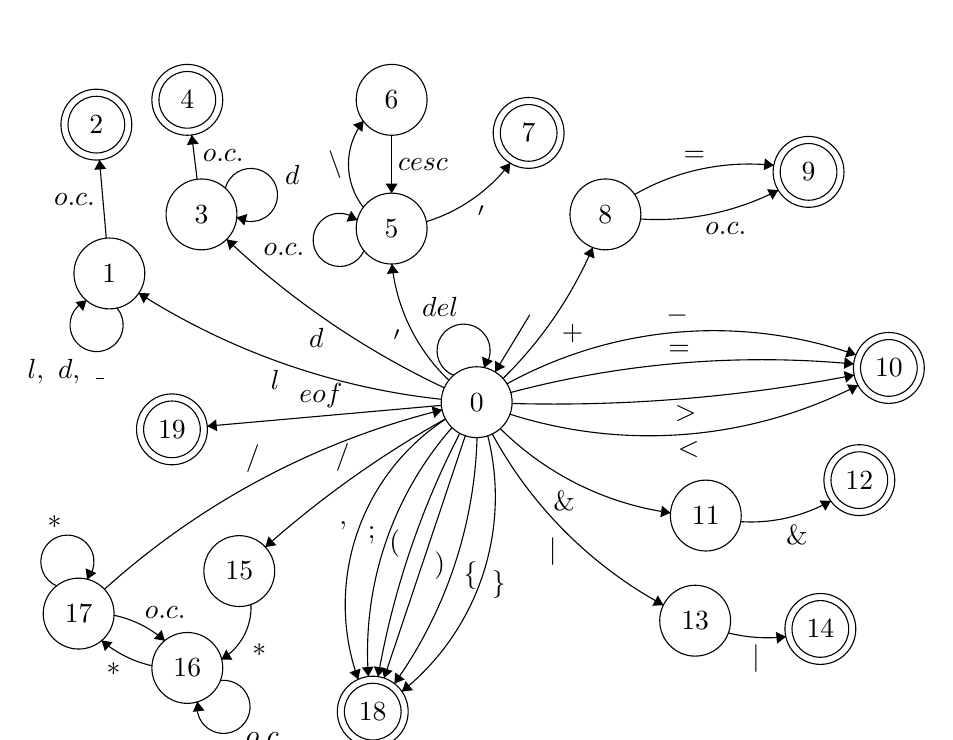
\begin{tikzpicture}[scale=0.15]
\tikzstyle{every node}+=[inner sep=0pt]
\draw [black] (38.4,-29.3) circle (3);
\draw (38.4,-29.3) node {$0$};
\draw [black] (7.3,-18.4) circle (3);
\draw (7.3,-18.4) node {$1$};
\draw [black] (6.2,-5.8) circle (3);
\draw (6.2,-5.8) node {$2$};
\draw [black] (6.2,-5.8) circle (2.4);
\draw [black] (15.1,-13.4) circle (3);
\draw (15.1,-13.4) node {$3$};
\draw [black] (13.9,-3.7) circle (3);
\draw (13.9,-3.7) node {$4$};
\draw [black] (13.9,-3.7) circle (2.4);
\draw [black] (31.2,-14.6) circle (3);
\draw (31.2,-14.6) node {$5$};
\draw [black] (31.2,-3.7) circle (3);
\draw (31.2,-3.7) node {$6$};
\draw [black] (42.8,-6.5) circle (3);
\draw (42.8,-6.5) node {$7$};
\draw [black] (42.8,-6.5) circle (2.4);
\draw [black] (49.3,-13.4) circle (3);
\draw (49.3,-13.4) node {$8$};
\draw [black] (66.5,-9.8) circle (3);
\draw (66.5,-9.8) node {$9$};
\draw [black] (66.5,-9.8) circle (2.4);
\draw [black] (73.3,-26.4) circle (3);
\draw (73.3,-26.4) node {$10$};
\draw [black] (73.3,-26.4) circle (2.4);
\draw [black] (57.8,-38.9) circle (3);
\draw (57.8,-38.9) node {$11$};
\draw [black] (70.8,-35.9) circle (3);
\draw (70.8,-35.9) node {$12$};
\draw [black] (70.8,-35.9) circle (2.4);
\draw [black] (56.9,-47.8) circle (3);
\draw (56.9,-47.8) node {$13$};
\draw [black] (67.5,-48.5) circle (3);
\draw (67.5,-48.5) node {$14$};
\draw [black] (67.5,-48.5) circle (2.4);
\draw [black] (18.3,-43.6) circle (3);
\draw (18.3,-43.6) node {$15$};
\draw [black] (13.9,-51.8) circle (3);
\draw (13.9,-51.8) node {$16$};
\draw [black] (4.7,-47.2) circle (3);
\draw (4.7,-47.2) node {$17$};
\draw [black] (29.6,-55.5) circle (3);
\draw (29.6,-55.5) node {$18$};
\draw [black] (29.6,-55.5) circle (2.4);
\draw [black] (12.6,-31.6) circle (3);
\draw (12.6,-31.6) node {$19$};
\draw [black] (12.6,-31.6) circle (2.4);
\draw [black] (35.41,-29.054) arc (-96.15072:-122.4786:59.606);
\fill [black] (9.79,-20.07) -- (10.2,-20.93) -- (10.73,-20.08);
\draw (21.34,-26.57) node [below] {$l$};
\draw [black] (36.458,-27.028) arc (248.25582:-39.74418:2.25);
\draw (35.31,-22.12) node [above] {$del$};
\fill [black] (39.02,-26.38) -- (39.78,-25.82) -- (38.85,-25.45);
\draw [black] (42.9,-21.9) -- (39.96,-26.74);
\fill [black] (39.96,-26.74) -- (40.8,-26.31) -- (39.95,-25.79);
\draw [black] (7.04,-15.41) -- (6.46,-8.79);
\fill [black] (6.46,-8.79) -- (6.03,-9.63) -- (7.03,-9.54);
\draw (6.12,-12.17) node [left] {$o.c.$};
\draw [black] (7.94,-21.319) arc (40.10787:-247.89213:2.25);
\draw (3.61,-25.66) node [below] {$l,\mbox{ }d,\mbox{ }\_$};
\fill [black] (5.37,-20.68) -- (4.44,-20.82) -- (5.08,-21.58);
\draw [black] (35.659,-28.081) arc (-115.2029:-133.41663:70.465);
\fill [black] (17.23,-15.51) -- (17.47,-16.42) -- (18.16,-15.69);
\draw (24.83,-23.03) node [below] {$d$};
\draw [black] (17.112,-11.19) arc (165.42106:-122.57894:2.25);
\draw (22.13,-10.07) node [right] {$d$};
\fill [black] (18.08,-13.65) -- (18.73,-14.34) -- (18.98,-13.37);
\draw [black] (14.73,-10.42) -- (14.27,-6.68);
\fill [black] (14.27,-6.68) -- (13.87,-7.53) -- (14.86,-7.41);
\draw (15.17,-8.42) node [right] {$o.c.$};
\draw [black] (36.047,-27.446) arc (-133.65734:-174.15181:15.848);
\fill [black] (31.22,-17.6) -- (30.81,-18.44) -- (31.8,-18.34);
\draw (32.05,-24.04) node [left] {$'$};
\draw [black] (28.864,-16.463) arc (-23.69198:-311.69198:2.25);
\draw (23.86,-16.4) node [left] {$o.c.$};
\fill [black] (28.3,-13.88) -- (27.77,-13.1) -- (27.37,-14.02);
\draw [black] (28.826,-12.819) arc (-141.47856:-218.52144:5.89);
\fill [black] (28.83,-5.48) -- (27.94,-5.8) -- (28.72,-6.42);
\draw (27.04,-9.15) node [left] {$\backslash$};
\draw [black] (31.2,-6.7) -- (31.2,-11.6);
\fill [black] (31.2,-11.6) -- (31.7,-10.8) -- (30.7,-10.8);
\draw (31.7,-9.15) node [right] {$cesc$};
\draw [black] (41.24,-9.056) arc (-37.41152:-72.73715:14.277);
\fill [black] (41.24,-9.06) -- (40.36,-9.39) -- (41.15,-10);
\draw (38.8,-12.59) node [below] {$'$};
\draw [black] (48.233,-16.203) arc (-23.31516:-45.54881:34.871);
\fill [black] (48.23,-16.2) -- (47.46,-16.74) -- (48.38,-17.14);
\draw (45.57,-23.47) node [right] {$+$};
\draw [black] (51.777,-11.713) arc (119.84259:83.80039:19.447);
\fill [black] (63.55,-9.25) -- (62.81,-8.66) -- (62.7,-9.66);
\draw (56.84,-8.96) node [above] {$=$};
\draw [black] (63.934,-11.35) arc (-62.70739:-93.64964:22.333);
\fill [black] (63.93,-11.35) -- (62.99,-11.27) -- (63.45,-12.16);
\draw (59.5,-14.04) node [below] {$o.c.$};
\draw [black] (40.965,-27.747) arc (118.831:70.66911:36.333);
\fill [black] (70.51,-25.29) -- (69.92,-24.55) -- (69.59,-25.5);
\draw (55.37,-22.81) node [above] {$-$};
\draw [black] (54.811,-38.667) arc (-97.84966:-134.80692:25.367);
\fill [black] (54.81,-38.67) -- (54.09,-38.06) -- (53.95,-39.05);
\draw (45.8,-36.78) node [below] {$\&$};
\draw [black] (68.375,-37.656) arc (-60.37001:-93.64076:13.669);
\fill [black] (68.38,-37.66) -- (67.43,-37.62) -- (67.93,-38.49);
\draw (65.51,-39.69) node [below] {$\&$};
\draw [black] (54.207,-46.479) arc (-118.50722:-151.49278:36.082);
\fill [black] (54.21,-46.48) -- (53.74,-45.66) -- (53.27,-46.54);
\draw (44.83,-40.76) node [below] {$|$};
\draw [black] (64.579,-49.159) arc (-83.54324:-104.01316:13.736);
\fill [black] (64.58,-49.16) -- (63.73,-48.75) -- (63.84,-49.75);
\draw (62.04,-49.78) node [below] {$|$};
\draw [black] (20.506,-41.567) arc (131.66584:119.19351:86.147);
\fill [black] (20.51,-41.57) -- (21.44,-41.41) -- (20.77,-40.66);
\draw (27.04,-35.23) node [above] {$/$};
\draw [black] (6.881,-45.141) arc (132.06374:103.88692:66.499);
\fill [black] (35.47,-29.95) -- (34.58,-29.66) -- (34.82,-30.63);
\draw (19.45,-35.28) node [above] {$/$};
\draw [black] (19.291,-46.387) arc (2.91612:-59.35083:5.157);
\fill [black] (16.77,-51.09) -- (17.71,-51.11) -- (17.2,-50.25);
\draw (19.36,-50.26) node [right] {$*$};
\draw [black] (10.918,-51.615) arc (-102.36433:-130.76577:9.753);
\fill [black] (6.64,-49.47) -- (6.92,-50.38) -- (7.57,-49.62);
\draw (7.65,-51.32) node [below] {$*$};
\draw [black] (7.684,-47.339) arc (78.23355:48.63635:9.442);
\fill [black] (12,-49.5) -- (11.73,-48.59) -- (11.07,-49.34);
\draw (12.03,-47.63) node [above] {$o.c.$};
\draw [black] (2.839,-44.862) arc (246.26123:-41.73877:2.25);
\draw (2.65,-40.02) node [above] {$*$};
\fill [black] (5.42,-44.3) -- (6.2,-43.77) -- (5.29,-43.37);
\draw [black] (35.41,-29.57) -- (15.59,-31.33);
\fill [black] (15.59,-31.33) -- (16.43,-31.76) -- (16.34,-30.76);
\draw (25.21,-29.8) node [above] {$eof$};
\draw [black] (28.368,-52.768) arc (-160.31098:-236.82114:18.77);
\fill [black] (28.37,-52.77) -- (28.57,-51.85) -- (27.63,-52.18);
\draw (27.48,-39.76) node [left] {$,$};
\draw [black] (29.231,-52.524) arc (-175.91406:-221.21806:28.862);
\fill [black] (29.23,-52.52) -- (29.67,-51.69) -- (28.68,-51.76);
\draw (29.89,-40.57) node [left] {$;$};
\draw [black] (30.052,-52.534) arc (170.14119:152.72669:71.764);
\fill [black] (30.05,-52.53) -- (30.68,-51.83) -- (29.7,-51.66);
\draw (31.96,-41.26) node [left] {$($};
\draw [black] (37.44,-32.14) -- (30.56,-52.66);
\fill [black] (30.56,-52.66) -- (31.28,-52.06) -- (30.34,-51.74);
\draw (34.77,-43.11) node [right] {$)$};
\draw [black] (38.432,-32.299) arc (-1.66748:-35.46464:37.795);
\fill [black] (31.44,-53.13) -- (32.31,-52.77) -- (31.49,-52.19);
\draw (37.25,-43.94) node [right] {$\{$};
\draw [black] (39.338,-32.147) arc (14.16948:-51.3016:21.117);
\fill [black] (32.07,-53.8) -- (33,-53.69) -- (32.38,-52.91);
\draw (39.65,-44.75) node [right] {$\}$};
\draw [black] (41.285,-28.477) arc (104.87742:84.62269:82.844);
\fill [black] (70.32,-26.06) -- (69.57,-25.49) -- (69.48,-26.49);
\draw (55.55,-25.41) node [above] {$=$};
\draw [black] (70.686,-27.871) arc (-62.84962:-107.65027:38.794);
\fill [black] (70.69,-27.87) -- (69.75,-27.79) -- (70.2,-28.68);
\draw (56.34,-32.59) node [below] {$<$};
\draw [black] (70.362,-27.007) arc (-78.97548:-91.52441:132.966);
\fill [black] (70.36,-27.01) -- (69.48,-26.67) -- (69.67,-27.65);
\draw (56.09,-29.58) node [below] {$>$};
\draw [black] (16.693,-52.862) arc (96.92389:-191.07611:2.25);
\draw (20.58,-57.23) node [below] {$o.c.$};
\fill [black] (14.76,-54.66) -- (14.36,-55.52) -- (15.35,-55.4);
\end{tikzpicture}
\end{center}


\section{Acciones semánticas}
A lo largo de esta sección, describimos las acciones semánticas que hemos añadido a las transiciones del Autómata Finito Determinista. Estas acciones permiten que se lleven a cabo acciones como la lectura, la identificación de los tokens o, en su lugar, una correcta gestión de los errores léxicos. A continuación, detallamos las operaciones utilizadas y, por legibilidad en el AFD, las transiciones en las que se realiza cada una:\\
\begin{tabbing}
    \hspace{1cm}\=\hspace{4.5cm}\=\hspace{2cm}\=\hspace{1cm}\=\hspace{1cm}\=\kill
    \>0. P' → \textbf{\{TSG := CrearTS(); TSL := NULL; DespG := 0\}} P \textbf{\{DestruirTS(TSG)\}}\\
    \>1. P → FUNCTION P\\
    \>2. P → STATEMENT P\\
    \>3. P → $eof$\\
    \>4. FUNCTION → function FUNTYPE $id$ \textbf{\{TSL := CrearTS(); DespL := 0\}} \\
    \>              \>( FUNATTRIBUTES ) \textbf{\{InsertaTipoTS(id.pos, }\\
    \>              \> \textbf{FUNATTRIBUTES.tipo → FUNTYPE.tipo);}\\
    \>           \>\textbf{InsertaEtiquetaTS(id.pos, nueva\_etiqueta())\}}\\
    \>              \>\{ BODY \}\> \textbf{\{if (BODY.tipo != tipo\_ok) then error(000) }\\
    \>              \>          \> \textbf{ if (FUNTYPE.tipo != BODY.tipoRet)}\\
    \>              \>          \>             \>   \textbf{then error(101)}\\
    \>              \>          \> \textbf{DestruirTS(TSL)\}}\\
    \>5. FUNTYPE → $void$ \textbf{\{FUNTYPE.tipo := void\}}\\
    \>6. FUNTYPE → VARTYPE \textbf{\{FUNTYPE.tipo := VARTYPE.tipo\}}\\
    \>7. VARTYPE → $int$ \textbf{\{VARTYPE.tipo := int; := VARTYPE.ancho := 1\}}\\
    \>8. VARTYPE → $boolean$ \textbf{\{VARTYPE.tipo := log; := VARTYPE.ancho := 1\}}\\
    \>9. VARTYPE → $string$ \textbf{\{VARTYPE.tipo := str; := VARTYPE.ancho := 64\}}\\
    \>10. FUNATTRIBUTES → $void$ \textbf{\{FUNATTRIBUTES.tipo := void\}}\\
    \>11. FUNATTRIBUTES → \>VARTYPE $id$ \textbf{\{
    if(BuscaTipoTS(id.pos) != NULL)} \\
    \>              \>          \>
    \>\textbf{then error(000)}\\
    \>              \>          \>
    \textbf{\{InsertaTipoTS(id.pos, VARTYPE.tipo);}\\
    \>                    \>        \>\textbf{InsertaDespTS(id.pos, DespL);}\\
    \>                    \>        \>\textbf{DespL := DespL + VARTYPE.tipo\}}\\
    \>                    \>NEXTATTRIBUTE \textbf{\{FUNATTRIBUTES.tipo :=}\\
    \>                    \>                      \> \textbf{if (NEXTATTRIBUTE.tipo != void) then}\\
    \>                    \>                      \> \>\textbf{VARTYPE.tipo × NEXTATTRIBUTE.tipo}\\
    \>                    \>                      \> \textbf{else VARTYPE.tipo\}}\\
    \>12. NEXTATTRIBUTE → , VARTYPE $id$ \textbf{\{
    if(BuscaTipoTS(id.pos) != NULL)} \\
    \>              \>          \>
    \>\textbf{then error(000)}\\
    \>              \>          \>
    \textbf{\{InsertaTipoTS(id.pos, VARTYPE.tipo);}\\
    \>                    \>        \>\textbf{InsertaDespTS(id.pos, DespL);}\\
    \>                    \>        \>\textbf{DespL := DespL + VARTYPE.tipo\}}\\
    \>                    \>NEXTATTRIBUTE$_1$ \textbf{\{NEXTATTRIBUTE.tipo :=}\\
    \>                    \>                      \> \textbf{if (NEXTATTRIBUTE$_1$.tipo != void) then}\\
    \>                    \>                      \> \>\textbf{VARTYPE.tipo $\times$ NEXTATTRIBUTE$_1$.tipo}\\
    \>                    \>                      \> \textbf{else VARTYPE.tipo\}}\\
    \>13. NEXTATTRIBUTE → $\lambda$ \textbf{\{NEXTATTRIBUTE.tipo := void\}}\\
    \>14. BODY → STATEMENT BODY$_1$\\
    \>                    \>\textbf{\{BODY.tipo := if (STATEMENT.tipo = tipo\_ok)}\\
    \>                    \>           \>          \>\textbf{then BODY$_1$.tipo}\\
    \>                    \>           \>\textbf{else tipo\_error}\\
    \>                    \>\textbf{BODY.tipoRet := if(STATEMENT.tipoRet = BODY$_1$.tipoRet}\\
    \>                    \>           \>\textbf{or STATEMENT.tipoRet = void) then}\\
    \>                    \>           \>          \>\textbf{BODY$_1$.tipoRet}\\
    \>                    \>           \>\textbf{else if (BODY$_1$.tipoRet = void) then}\\
    \>                    \>           \>          \>\textbf{STATEMENT.tipoRet}\\
    \>                    \>           \>\textbf{else tipo\_error\}}\\
    \>15. BODY → $\lambda$ \textbf{\{BODY.tipo := tipo\_ok; BODY.tipoRet := void\}}\\
    \>16. STATEMENT → $if$ ( EXP1 ) ATOMSTATEMENT\\
    \>                    \> \textbf{\{STATEMENT.tipo := if (EXP1.tipo != log)}\\
    \>                    \> \> \>\textbf{then tipo\_error}\\
    \>                    \> \> \textbf{else ATOMSTATEMENT.tipo}\\
    \>                    \> \textbf{STATEMENT.tipoRet := ATOMSTATEMENT.tipoRet\}}\\
    \\
    \\
    \>17. STATEMENT → $for$ ( FORACT$_1$ ; EXP1 ; FORACT$_2$ ) \{ BODY \}\\
    \>                    \> \textbf{\{STATEMENT.tipo := if (FORACT$_1$.tipo = tipo\_ok}\\
    \>                    \> \>\textbf{and EXP1.tipo = log and FORACT$_2$.tipo = tipo\_ok)}\\
    \>                    \> \> \>\textbf{then BODY.tipo}\\
    \>                    \> \>\textbf{else error(103)}\\
    \>                    \> \textbf{STATEMENT.tipoRet := BODY.tipoRet\}}\\
    \>18. STATEMENT → $var$ VARTYPE $id$ ; \textbf{\{if(BuscaTipoTS(id.pos) != NULL)} \\
    \>              \>          \>
    \>\textbf{then error(000)}\\
    \>                    \> \textbf{insertaTipoTS(id.pos, VARTYPE.tipo)}\\
    \>                    \> \textbf{if(TSL != NULL) then }\\
    \>                    \> \> \textbf{insertaDespTS(id.pos,despG)}\\
    \>                    \> \> \textbf{despG := despG + VARTYPE.ancho}\\
    \>                    \> \textbf{else}\\
    \>                    \> \> \textbf{insertaDespTS(id.pos,despL)}\\
    \>                    \> \> \textbf{despL := despL + VARTYPE.ancho}\\
    \>                    \> \textbf{STATEMENT.tipo := tipo\_ok\}}\\
    \>19. STATEMENT → ATOMSTATEMENT \textbf{\{STATEMENT.tipo := ATOMSTATEMENT.tipo}\\
    \>                    \> \textbf{STATEMENT.tipoRet := ATOMSTATEMENT.tipoRet\}}\\

    \>20. ATOMSTATEMENT → $id$ IDACT ; \> \> \textbf{\{if(IDACT.funCall)\{}\\
    \> \> \> \textbf{if (id.tipo != R $\rightarrow$ T) then}\\
    \> \> \> \> \textbf{ATOMSTATEMENT.tipo := tipo\_error}\\
    \> \> \> \> \textbf{error(201)}\\
    \> \> \> \textbf{else if (IDACT.tipo = tipo\_error)}\\
    \> \> \> \> \textbf{then ATOMSTATEMENT = tipo\_error}\\
    \> \> \> \textbf{else if (IDACT.tipo = R.tipo)}\\
    \> \> \> \> \textbf{then ATOMSTATEMENT = tipo\_ok}\\
    \> \> \> \textbf{else}\\
    \> \> \> \> \textbf{ATOMSTATEMENT = tipo\_error}\\
    \> \> \> \> \textbf{error(203)}\\
    \> \> \textbf{\} else \{}\\
    \> \> \> \textbf{if (id.tipo = R $\rightarrow$ T) then}\\
    \> \> \> \> \textbf{ATOMSTATEMENT.tipo := tipo\_error}\\
    \> \> \> \> \textbf{error(202)}\\
    \> \> \> \textbf{else if (IDACT.tipo = tipo\_error)}\\
    \> \> \> \> \textbf{then ATOMSTATEMENT = tipo\_error}\\
    \> \> \> \textbf{else if (IDACT.tipo = R.tipo)}\\
    \> \> \> \> \textbf{then ATOMSTATEMENT = tipo\_ok}\\
    \> \> \> \textbf{else}\\
    \> \> \> \> \textbf{ATOMSTATEMENT = tipo\_error}\\
    \> \> \> \> \textbf{error(200)}\\
    \>21. ATOMSTATEMENT → $output$ EXP1 ; \textbf{\{if (EXP1.tipo $\in$ \{int, str\}) then}\\
    \>                    \> \> \> \textbf{ATOMSTATEMENT.tipo := tipo\_ok}\\
    \>                    \> \>\textbf{else} \\
    \> \> \> \textbf{ATOMSTATEMENT.tipo := tipo\_error}\\
    \> \> \> \textbf{error(104)}\\
    \>                    \> \textbf{ATOMSTATEMENT.tipoRet := void\}}\\
    \>22. ATOMSTATEMENT → $input$ $id$ ; \textbf{\{if (buscaTipoTS(id.pos) $\in$ \{int, str\})}\\
    \>                    \> \>\textbf{then ATOMSTATEMENT.tipo := tipo\_ok}\\
    \>                    \> \textbf{else} \\
    \> \> \> \textbf{ATOMSTATEMENT.tipo := tipo\_error}\\
    \> \> \> \textbf{error(105)}\\
    \>                    \> \textbf{ATOMSTATEMENT.tipoRet := void\}}\\
    \>23. ATOMSTATEMENT → $return$ RETURNEXP ; \textbf{\{ATOMSTATEMENT.tipo :=}\\
    \>                    \> \textbf{if (RETURNEXP.tipo != tipo\_error) then tipo\_ok}\\
    \>                    \> \textbf{else tipo\_error}\\
    \>                    \> \textbf{ATOMSTATEMENT.tipoRet := RETURNEXP.tipo\}}\\
    \\
    \>24. IDACT → ASS EXP1 \textbf{\{IDACT.tipo :=}\\
    \>                    \> \textbf{if ((ASS.sum = true AND EXP1.tipo $\in$ \{int, str\})}\\
    \>                    \> \>\textbf{OR ASS.sum = false) then EXP1.tipo}\\
    \>                    \> \textbf{else tipo\_error\}}\\
    \>25. IDACT → ( CALLPARAM ) \textbf{\{IDACT.tipo := CALLPARAM.tipo\}}\\
    \>26. FORACT → $id$ ASS EXP1 \textbf{\{if (buscaTipoTS(id.pos) != int)}\\
    \> \> \> \textbf{FORACT.tipo := tipo\_error}\\
    \> \> \> \textbf{error(102)}\\
    \> \> \textbf{else if EXP1.tipo = tipo\_error}\\
    \> \> \> \textbf{FORACT.tipo := tipo\_error}\\
    \> \> \textbf{else if EXP1.tipo != int} \\
        \> \> \> \textbf{FORACT.tipo := tipo\_error}\\
    \> \> \> \textbf{error(200)}\\
    \> \> \textbf{else FORACT.tipo := tipo\_ok}\\
    \>27. FORACT → $\lambda$ \textbf{\{FORACT.tipo := tipo\_ok\}}\\
    \>28. ASS → = \textbf{\{ASS.sum = false\}}\\
    \>29. ASS → += \textbf{\{ASS.sum = true\}}\\
    \>30. CALLPARAM → EXP1 NEXTPARAM \textbf{\{CALLPARAM.tipo :=}\\
    \>                    \> \textbf{if (EXP1.tipo = tipo\_error}\\
    \>                    \> \textbf{OR NEXTPARAM.tipo == tipo\_error) then}\\
    \>                    \> \> \textbf{tipo\_error}\\
    \>                    \> \textbf{else if (NEXTPARAM.tipo != void) then}\\
    \>                    \> \>\textbf{EXP1.tipo $\times$ NEXTPARAM.tipo}\\
    \>                    \> \textbf{else tipo\_error\}}\\ 
    \>31. CALLPARAM → $\lambda$ \textbf{\{CALLPARAM.tipo := void\}}\\
    \>32. NEXTPARAM → , EXP1 NEXTPARAM$_1$ \textbf{\{CALLPARAM.tipo :=}\\
    \>                    \> \textbf{if (EXP1.tipo = tipo\_error}\\
    \>                    \> \textbf{OR NEXTPARAM$_1$.tipo == tipo\_error) then}\\
    \>                    \> \> \textbf{tipo\_error}\\
    \>                    \> \textbf{else if (NEXTPARAM$_1$.tipo != void) then}\\
    \>                    \> \>\textbf{EXP1.tipo $\times$ NEXTPARAM$_1$.tipo}\\
    \>                    \> \textbf{else tipo\_error\}}\\ 
    \>33. NEXTPARAM → $\lambda$ \textbf{\{NEXTPARAM.tipo := void\}}\\
    \>34. RETURNEXP → EXP1 \textbf{RETURNEXP.tipo := EXP1.tipo}\\
    \>35. RETURNEXP → $\lambda$ \textbf{RETURNEXP.tipo := void}\\
    \>36. EXP1 → EXP2 EXPOR \>\textbf{\{if (EXPOR.tipo = void) then EXP1.tipo := EXP2.tipo}\\
    \>                     \> \textbf{else if (EXP2.tipo != log OR EXPOR.tipo = tipo\_error) then}\\
    \>                     \> \> \textbf{error(100)}\\
    \>                     \> \> \textbf{EXP1.tipo := tipo\_error}\\
    \>                     \> \textbf{else EXP1.tipo := log\}}\\
    \>37. EXPOR → \verb!||! EXP2 EXPOR$_1$\\
    \>                     \>\textbf{\{if (EXP2.tipo != log OR EXPOR$_1$.tipo = tipo\_error) then}\\
    \>                     \> \> \textbf{error(100)}\\
    \>                     \> \> \textbf{EXPOR.tipo := tipo\_error}\\
    \>                     \> \textbf{else EXPOR.tipo := logico\}}\\
    \>38. EXPOR → $\lambda$ \textbf{\{EXPOR.tipo := void\}}\\
    \>39. EXP2 → EXP3 EXPAND\\
    \>                     \>\textbf{\{if (EXPAND.tipo = void) then EXP2.tipo := EXP3.tipo}\\
    \>                     \> \textbf{else if (EXP3.tipo != log OR EXPAND.tipo = tipo\_error) then}\\
    \>                     \> \> \textbf{error(100)}\\
    \>                     \> \> \textbf{EXP2.tipo := tipo\_error}\\
    \>                     \> \textbf{else EXP2.tipo := log\}}\\
    \>40. EXPAND → \verb!&&! EXP3 EXPAND$_1$\\
    \>                     \>\textbf{\{if (EXP3.tipo != log OR EXPAND$_1$.tipo = tipo\_error) then}\\
    \>                     \> \> \textbf{error(100)}\\
    \>                     \> \> \textbf{EXPAND.tipo := tipo\_error}\\
    \>                     \> \textbf{else EXPAND.tipo := logico\}}\\
    \>41. EXPAND → $\lambda$ \textbf{\{EXPAND.tipo := void\}}\\
    \\
    \>42. EXP3 → EXP4 COMP \>\textbf{\{if (COMP.tipo = void) then EXP3.tipo := EXP4.tipo}\\
    \>                     \> \textbf{else if (EXP4.tipo != int OR COMP.tipo = tipo\_error) then}\\
    \>                     \> \> \textbf{error(100)}\\
    \>                     \> \> \textbf{EXP3.tipo := tipo\_error}\\
    \>                     \> \textbf{else EXP3.tipo := log\}}\\
    \>43. COMP → COMPOP EXP4 COMP$_1$\\
    \>                     \>\textbf{\{if (EXP4.tipo != int OR COMP$_1$.tipo = tipo\_error) then}\\
    \>                     \> \> \textbf{error(100)}\\
    \>                     \> \> \textbf{COMP.tipo := tipo\_error}\\
    \>                     \> \textbf{else COMP.tipo := logico\}}\\
    \>44. COMP → $\lambda$ \textbf{\{COMP.tipo := void\}}\\
    \>45. COMPOP → >\\
    \>46. COMPOP → <\\
    \>47. EXP4 → EXPATOM ARITH\\
    \>                     \>\textbf{\{if (ARITH.tipo = void) then EXP4.tipo := EXPATOM.tipo}\\
    \>                     \>\textbf{\{else if (EXPATOM.tipo != int AND EXPATOM.tipo != string) then}\\
    \> \> \> \textbf{EXP4.tipo := tipo\_error}\\
    \> \> \> \textbf{error(100)}\\
    \>                     \> \textbf{else if (ARITH.tipo = tipo\_error) then EXP4.tipo := tipo\_error}\\
    \>                     \> \textbf{else if (EXPATOM != ARITH.tipo) then}\\ 
    \> \> \> \textbf{EXP4.tipo := tipo\_error}\\
    \>                     \> \> \textbf{error(200)}\\
    \>                     \> \textbf{else EXP4.tipo := ARITH.tipo\}}\\
    \>48. ARITH → ARITHOP EXPATOM ARITH$_1$\\
    \>                     \>\textbf{\{if (ARITHOP.sum = false AND EXPATOM.tipo != int) then}\\
    \>                     \> \> \textbf{ARITH.tipo := tipo\_error}\\
    \>                     \> \> \textbf{error(100)}\\
    \> \>\textbf{else if (ARITHOP.sum = true AND EXPATOM.tipo != int}\\
    \> \> \>\textbf{AND EXPATOM.tipo != string) then}\\     
    \> \> \> \> \textbf{ARITH.tipo := tipo\_error}\\
    \> \> \> \> \textbf{error(100)}\\
    \>                     \> \textbf{else if (ARITH$_1$.tipo = tipo\_error)}\\     \> \> \> \textbf{ARITH.tipo := tipo\_error}\\
    \>                     \> \textbf{else if (ARITH$_1$.tipo != void AND EXPATOM.tipo != ARITH$_1$.tipo) then}\\ 
    \> \> \> \textbf{ARITH.tipo := tipo\_error}\\
    \>                     \> \> \textbf{error(200)}\\
    \>                     \> \textbf{else ARITH.tipo := EXPATOM.tipo\}}\\
    \>49. ARITH → $\lambda$ \textbf{\{ARITH.tipo := void\}}\\
    \>50. ARITHOP → +\\
    \>51. ARITHOP → -\\
    \>52. EXPATOM → $id$ IDVAL \textbf{\{if(IDVAL.funCall)\{}\\
    \> \> \> \textbf{if (id.tipo != R $\rightarrow$ T) then}\\
    \> \> \> \> \textbf{EXPATOM.tipo := tipo\_error}\\
    \> \> \> \> \textbf{error(201)}\\
    \> \> \> \textbf{else if (IDVAL.tipo = tipo\_error)}\\
    \> \> \> \> \textbf{then EXPATOM = tipo\_error}\\
    \> \> \> \textbf{else if (IDVAL.tipo = R.tipo)}\\
    \> \> \> \> \textbf{then EXPATOM = T.tipo}\\
    \> \> \> \textbf{else}\\
    \> \> \> \> \textbf{EXPATOM = tipo\_error}\\
    \> \> \> \> \textbf{error(203)}\\
    \> \> \textbf{\} else \{}\\
    \> \> \> \textbf{if (id.tipo = R $\rightarrow$ T) then}\\
    \> \> \> \> \textbf{EXPATOM.tipo := tipo\_error}\\
    \> \> \> \> \textbf{error(202)}\\
    \> \> \> \textbf{else}\\
    \> \> \> \> \textbf{EXPATOM = id.tipo}\\
    \>53. EXPATOM → ( EXP1 ) \>\textbf{\{EXPATOM.tipo := EXP1.tipo\}}\\
    \>54. EXPATOM → cint \>\textbf{\{EXPATOM.tipo := int\}}\\
    \>55. EXPATOM → cstr \>\textbf{\{EXPATOM.tipo := str\}}\\
    \>56. EXPATOM → true \>\textbf{\{EXPATOM.tipo := log\}}\\
    \>57. EXPATOM → false \>\textbf{\{EXPATOM.tipo := log\}}\\
    \>58. IDVAL → ( CALLPARAM )\\
    \>59. IDVAL → $\lambda$\\
\end{tabbing}

\section{Gestión de errores}
Los casos de error posibles son todas aquellas transiciones no recogidas por nuestro AFD. En estos casos, se generará un error léxico y se informará al usuario de la existencia de un error en el código fuente, junto con el número de línea y columna en la que se ha detectado el mismo. A continuación, detallamos los errores que hemos identificado y los mensajes de error correspondientes a cada uno:\\
\begin{itemize}[left=1cm]
    \item \textbf{Caracteres no reconocidos.} En caso de que el carácter leído no coincida con ninguna transición del AFD, de manera que no pueda transitar desde el estado 0, se generará un error léxico con el siguiente mensaje: \textcolor{red}{(línea:columna) ERROR: Carácter inesperado al buscar el siguiente símbolo («carácter inesperado», U+20AC).}
    \item \textbf{Comentario de bloque mal abierto.} En caso de que tras encontrar una `/' no se encuentre un «*», se generará un error léxico con el siguiente mensaje: \textcolor{red}{(línea:columna) ERROR: Carácter inesperado tras «/». Se esperaba «*» para abrir un comentario de bloque}
    \item \textbf{Comentario de bloque no cerrado.} Si se detecta un comentario de bloque sin cerrar, se generará un error léxico con el siguiente mensaje: \textcolor{red}{(línea:columna) ERROR: Fin de fichero inesperado. Se esperaba «*/» para cerrar el comentario de bloque.}
    \item \textbf{Valor entero fuera de rango.} Si el valor de una constante entera supera el rango permitido que abarcan los enteros de 16 bits con signo, se generará un error léxico con el siguiente mensaje: \textcolor{red}{(línea:columna) ERROR: El valor del entero es demasiado grande. Rango permitido: [-32768, 32767].}
    \item \textbf{Cadena de caracteres no cerrada.} Si se detecta una cadena de caracteres sin cerrar, se generará un error léxico con el siguiente mensaje: \textcolor{red}{(línea:columna) ERROR: Fin de fichero inesperado. Se esperaba «'» para cerrar la cadena.}
    \item \textbf{Secuencia de escape no válida.} En este caso, distinguiremos dos situaciones:
    \begin{itemize}
        \item \textbf{Caracter imprimible tras la barra invertida.} Si el carácter siguiente a la barra invertida es un carácter imprimible, pero no forma ninguna secuencia de escape válida, se generará un error léxico con el siguiente mensaje: \textcolor{red}{(línea:columna) ERROR: en la cadena, la secuencia de escape «\textbackslash carácter» (U+{:04X}) no es válida.}
        \item \textbf{Caracter ilegal tras la barra invertida.} Si el carácter que sigue a la barra invertida no es un carácter imprimible, se generará un error léxico con el siguiente mensaje: \textcolor{red}{(línea:columna) ERROR: en la cadena, carácter ilegal en la secuencia de escape (U+{:04X}).}
    \end{itemize}
    \item \textbf{Carácter no permitido en la cadena.} Si se detecta un carácter no permitido en la cadena, como un salto de línea, se generará un error léxico con el siguiente mensaje: \textcolor{red}{(línea:columna) ERROR: en la cadena, carácter no permitido (U+{:04X}).}
    \item \textbf{Cadena de caracteres demasiado larga.} Si la longitud de la cadena supera los 64 caracteres, se generará un error léxico con el siguiente mensaje (donde x es el número de caracteres de la cadena): \textcolor{red}{(línea:columna) ERROR: La longitud de cadena excede el límite de 64 caracteres (x caracteres).}
    \item \textbf{Operadores lógicos incorrectos.} En caso de haber un \verb!&! en lugar de \verb!&&! o un \verb!|! en lugar de \verb!||!, se generará un error léxico con el siguiente mensaje (donde op será \verb!&! o \verb!|!): \textcolor{red}{(línea:columna) ERROR: Se esperaba «op» después de «op» para formar un operador.}
\end{itemize}

Para ilustrar mejor el comportamiento del programa, en la sección 8 presentamos varios casos en los que demostramos cómo el analizador maneja la detección de errores.

\section{Tabla de Símbolos}
Dado que en esta parte de la práctica solo se debe implementar el analizador léxico, nuestra tabla de símbolos es única y global. Por el momento, simplemente almacena los identificadores que el analizador léxico encuentre, y carecerá de atributos más allá del nombre del propio identificador.

\section{Funcionamiento del programa}
El programa que hemos elaborado comienza leyendo el código fuente que le proporcionamos. Lo analiza carácter por carácter, reconociendo los tokens que hemos definido en el punto 2. Para ello, el Analizador Léxico se basa en la gramática regular que genera nuestro Autómata Finito Determinista.

A medida que encuentra identificadores los almacena en la tabla de símbolos. Si encuentra delimitadores o comentarios de bloque, los ignora. Además, el programa está preparado para detectar errores, generando mensajes claros que indican el tipo y la ubicación exacta, con tal de facilitar la corrección por parte del usuario. Al finalizar la ejecución, queda completo un informe con todos los tokens que el programa ha reconocido durante el análisis, o los posibles errores que haya encontrado.

En el \textbf{anexo} es posible encontrar distintos casos que demuestran el funcionamiento correcto del programa. Los tres primeros son favorables y los tres últimos muestran distintos casos de error. A continuación incluimos una breve explicación de cada uno:

\begin{itemize}
    \item \textbf{Caso 1:} El programa reconoce declaraciones válidas, como la asignación de tipos a variables y la asignación de identificadores, como lo que ocurre con el tipo «boolean» (tratado como un identificador).
    
    \item \textbf{Caso 2:} Muestra el funcionamiento adecuado de una función println (para imprimir mensajes), con lo que se puede apreciar la correcta gestión de cadenas y el uso de saltos de línea.
    
    \item \textbf{Caso 3:} Demuestra la capacidad del programa para comparar variables de entrada y ejecutar operaciones matemáticas.
    
    \item \textbf{Caso 4:} Ilustra un error léxico causado por un comentario de bloque no cerrado, que resulta en un fin de fichero inesperado.
    
    \item \textbf{Caso 5:} Muestra que hay caracteres no permitidos al inicio de un token y que se produce un error si declaramos variables que no cumplen con las convenciones, como empezar por «\_».
    
    \item \textbf{Caso 6:} Resalta cómo el programa continúa buscando tokens válidos a pesar de haber errores en el código, lo que permite depurar varios errores en una sola ejecución.
\end{itemize}

Con esto, demostramos el funcionamiento del programa en diferentes situaciones, desde el reconocimiento de declaraciones válidas hasta la gestión de errores léxicos. Estos resultados serán completados gracias a la segunda entrega del proyecto, que se centrará en el desarrollo del Analizador Sintáctico.

\appendix
\section*{Anexo}

\lstset{
  language=C,
  basicstyle=\ttfamily\scriptsize,
  keywordstyle=,
  showstringspaces=false,
  escapeinside={(*@}{@*)},
}

\begin{enumerate}

    \item \textbf{Caso 1:} Funcionamiento correcto
    \begin{tcolorbox}[title={Código fuente}, colback=white]
        \begin{lstlisting}
/* Declaraciones válidas */
var boolean a;
var int b;
var string d;

/* Se vuelve a declarar la variable «a», pero no es error léxico. */
var int a;

/* El tipo «bool» no existe, se trata como identificador. */
var bool err;
        \end{lstlisting}
    \end{tcolorbox}

    \begin{tcolorbox}[title={Volcado del fichero de tokens}, colback=white]
        \begin{lstlisting}
<var, >
<bool, >
<id, 0>
<scol, >
<var, >
<int, >
<id, 1>
<scol, >
<var, >
<str, >
<id, 2>
<scol, >
<var, >
<int, >
<id, 0>
<scol, >
<var, >
<id, 3>
<id, 4>
<scol, >
<eof, >
        \end{lstlisting}
    \end{tcolorbox}

    \begin{tcolorbox}[title={Volcado del fichero de la tabla de símbolos}, colback=white]
        \begin{lstlisting}
Tabla Global #0:
*'a'
*'b'
*'d'
*'bool'
*'err'
        \end{lstlisting}
    \end{tcolorbox}


    \item \textbf{Caso 2:} Funcionamiento correcto
    \begin{tcolorbox}[title={Código fuente}, colback=white]
        \begin{lstlisting}
function void println(string s) {
    output s;
    output '\n';
}

println('¡Hola mundo!');
println('Eso son llamadas a \'output\' usando una función.');
        \end{lstlisting}
    \end{tcolorbox}

    \begin{tcolorbox}[title={Volcado del fichero de tokens}, colback=white]
        \begin{lstlisting}
<fn, >
<void, >
<id, 0>
<po, >
<str, >
<id, 1>
<pc, >
<cbo, >
<out, >
<id, 1>
<scol, >
<out, >
<cstr, "\n">
<scol, >
<cbc, >
<id, 0>
<po, >
<cstr, "¡Hola mundo!">
<pc, >
<scol, >
<id, 0>
<po, >
<cstr, "Eso son llamadas a \'output\' usando una función.">
<pc, >
<scol, >
<eof, >
        \end{lstlisting}
    \end{tcolorbox}

    \begin{tcolorbox}[title={Volcado del fichero de la tabla de símbolos}, colback=white]
        \begin{lstlisting}
Tabla Global #0:
*'println'
*'s'
        \end{lstlisting}
    \end{tcolorbox}


    \item \textbf{Caso 3:} Funcionamiento correcto
    \begin{tcolorbox}[title={Código fuente}, colback=white]
        \begin{lstlisting}
/* Leemos dos números del usuario. Las variables sin declarar se suponen globales y enteras. */
input a;
input b;

/* Comparamos los números entre sí. */
if (a < b) {
    output '\'a\' es menor que \'b\'.';
}
if (a > b) {
    output '\'a\' es mayor que \'b\'.';
}

output '\n';

/* Operamos con los números. */

output 'a + b: ';
output a + b;

output 'a - b: ';
output a - b;

output '\n';
        \end{lstlisting}        
    \end{tcolorbox}

    \begin{tcolorbox}[title={Volcado del fichero de tokens}, colback=white]
        \begin{lstlisting}
<in, >
<id, 0>
<scol, >
<in, >
<id, 1>
<scol, >
<if, >
<po, >
<id, 0>
<ls, >
<id, 1>
<pc, >
<cbo, >
<out, >
<cstr, "\'a\' es menor que \'b\'.">
<scol, >
<cbc, >
<if, >
<po, >
<id, 0>
<gr, >
<id, 1>
<pc, >
<cbo, >
<out, >
<cstr, "\'a\' es mayor que \'b\'.">
<scol, >
<cbc, >
<out, >
<cstr, "\n">
<scol, >
<out, >
<cstr, "a + b: ">
<scol, >
<out, >
<id, 0>
<sum, >
<id, 1>
<scol, >
<out, >
<cstr, "a - b: ">
<scol, >
<out, >
<id, 0>
<sub, >
<id, 1>
<scol, >
<out, >
<cstr, "\n">
<scol, >
<eof, >
        \end{lstlisting}
    \end{tcolorbox}

    \begin{tcolorbox}[title={Volcado del fichero de la tabla de símbolos}, colback=white]
        \begin{lstlisting}
Tabla Global #0:
*'a'
*'b'
        \end{lstlisting}
    \end{tcolorbox}

    
    \item \textbf{Caso 4:} Funcionamiento erróneo
    \begin{tcolorbox}[title={Código fuente}, colback=white]
        \begin{lstlisting}
/* Un comentario de bloque sin cerrar es un error léxico, ya que se recibe un EOF inesperado.
        \end{lstlisting}      
    \end{tcolorbox}

    \begin{tcolorbox}[title={Errores detectados}, colback=white]
        \begin{lstlisting}
(2:1) ERROR: Fin de fichero inesperado. Se esperaba «*/» para cerrar el comentario de bloque.
        \end{lstlisting}
    \end{tcolorbox}


    \item \textbf{Caso 5:} Funcionamiento erróneo
    \begin{tcolorbox}[title={Código fuente}, colback=white]
        \begin{lstlisting}
/* Hay algunos símbolos por los que un token no puede empezar. */
$ % @ # ?

/* En especial, las variables no pueden empezar con «_». */
var int _error;
        \end{lstlisting}      
    \end{tcolorbox}

    \begin{tcolorbox}[title={Errores detectados}, colback=white]
        \begin{lstlisting}
(2:1) ERROR: Carácter inesperado al buscar el siguiente símbolo («$», U+0024).
(2:3) ERROR: Carácter inesperado al buscar el siguiente símbolo («%», U+0025).
(2:5) ERROR: Carácter inesperado al buscar el siguiente símbolo («@», U+0040).
(2:7) ERROR: Carácter inesperado al buscar el siguiente símbolo («#», U+0023).
(2:9) ERROR: Carácter inesperado al buscar el siguiente símbolo («?», U+003F).
(5:9) ERROR: Carácter inesperado al buscar el siguiente símbolo («_», U+005F).
        \end{lstlisting}
    \end{tcolorbox}

    
    \item \textbf{Caso 6:} Funcionamiento erróneo
    \begin{tcolorbox}[title={Código fuente}, colback=white]
        \begin{lstlisting}
/* Aunque el código esté malformado y no compile, se siguen buscando y generando tokens */
var string a = $ 'Esta cadena se lee correctamente';

/* Esto es útil para depurar los errores sin detenerse sólo en el primero. */
var int a = 2?;

/* En algunos casos, es imposible recuperar tokens en un estado válido y seguir procesando. */
var string s = 'Si no se temina el string, lee todo \'; $$ /**/;; Esto es parte de la cadena.
/* Aquí ya ha terminado la cadena, ya que lee un salto de línea no permitido. */

/* Como la última cadena ya finalizó por error, aquí se recupera y sigue procesando tokens. */
var string s2 = 'Esta cadena se procesa bien';
        \end{lstlisting}      
    \end{tcolorbox}

    \begin{tcolorbox}[title={Errores detectados}, colback=white]
        \begin{lstlisting}
(2:16) ERROR: Carácter inesperado al buscar el siguiente símbolo («$», U+0024).
(5:14) ERROR: Carácter inesperado al buscar el siguiente símbolo («?», U+003F).
(8:94) ERROR: Error en la cadena. Carácter no permitido (U+000D).
        \end{lstlisting}
    \end{tcolorbox}

\end{enumerate}


\end{document}
